\documentclass[11pt]{article}
\usepackage[margin=0.9in]{geometry}
\usepackage{amsmath,amssymb,booktabs,graphicx}
\usepackage[hidelinks]{hyperref}
\newcommand{\Tr}{\operatorname{Tr}}
\newcommand{\eps}{\epsilon}
\title{Hubbard architecture comparison: compilation, locality, and injection}
\author{Working research note: second refinement}
\date{22 September 2026}
\begin{document}
\maketitle

We refine the physical-qubit calculation and separate injected-state error from
physical gate error in the factory model. The shared task remains the central
doublon expectation after a half-filled N\'eel quench on an open square, with
$U/J=4$. The target is $1\%$ relative error at the provisional signal
$D_*=0.1$, hence $\eps=10^{-3}$, with $95\%$ statistical confidence. We retain
$\tau=1$ and the shared step count $r=4$ for the main comparison. The additional
$r=1$ calculations expose circuit locality; neither step count is certified
against the allocated Trotter bias. No Hubbard dynamics curve is simulated.

\section{Native gates and fermionic motion}
We extract number-conserving two-mode hopping, fermionic Hadamard, and density
blocks from the first compiled workload. Their noncommuting order is unchanged.
Our physical gate set contains arbitrary $R_{ZZ}(\phi)$ and one-qubit pulses,
each taking $10$~ns. A two-qubit depolarizing fault has total probability
$p=10^{-3}$; a one-qubit fault has probability $p/10$. The idle channel has
error $p$ per $100$~ns. These are explicit native-gate assumptions, not a
characterization of a particular device.

Fermionic swaps provide a way to bring interacting modes together~\cite{kivlichan2018}.
In the adjacent occupation basis, write
\begin{equation}
 V(\theta)=e^{-i\theta(XX+YY)},\qquad
 F_{\mathrm{swap}}=(S\otimes S)V(\pi/4).
\end{equation}
Thus $F_{\mathrm{swap}}V(\theta)$ requires the same two variable-angle
entanglers as $V(\theta+\pi/4)$, together with local phases. More generally,
a number-conserving Gaussian gate is specified by an odd-sector matrix
$G\in U(2)$; its vacuum amplitude is one and its double-occupancy amplitude
is $\det G$. We decompose
\begin{equation}
 G=e^{i\delta}R_z(\alpha)R_x(\beta)R_z(\gamma).
\end{equation}
Opposite one-qubit $Z$ rotations implement odd-sector $R_z$. Two native
entanglers implement the odd-sector $R_x$ through
\begin{equation}
 U_x(\beta)=e^{-i\beta XX/4}e^{-i\beta YY/4}.
\end{equation}
Equal final $Z$ rotations supply the determinant. Products of Gaussian gates on the same pair
therefore still require at most two $R_{ZZ}$ gates. Density rotations commute
with these pair gates and add at most one further $R_{ZZ}$.

We keep a live fermionic mode order and use only swaps adjacent in that order.
A small lookahead chooses which endpoint moves. Pair operations can fuse
through operations on disjoint wires. We select among four lookahead lengths
using the local-PEC cost under the declared noise model. This is a heuristic
compiler, not an optimal swap network. A separate implementation uses a
two-root parity tree on the physical square grid; it preserves the complete
Jordan--Wigner string and uses grid edges outside the original snake path.

The experimental comparison needs care. The Phasecraft/Quantinuum implementation
uses all-to-all connectivity to make ordinary SWAP a relabeling operation;
this lets an isolated fermionic swap use one entangler~\cite{alam2025}.
Our nearest-neighbor array must implement the mode motion. We therefore do
not use its gate count as a direct calibration of the array's routing cost.

\begin{figure}[t]
\centering
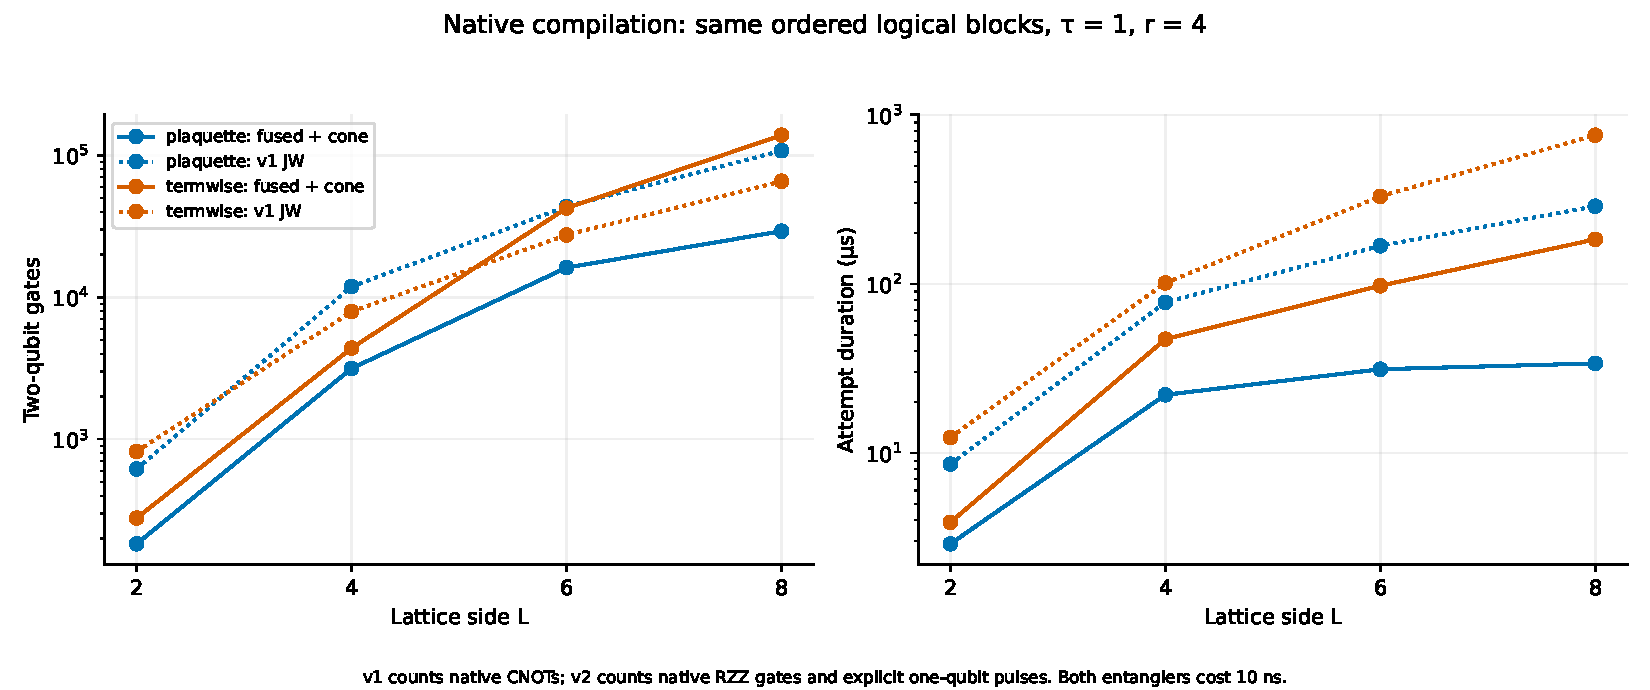
\includegraphics[width=\linewidth]{results/nisq_v2/native_compilation.pdf}
\caption{Actual CUDA-Q P0 counts and project-side ASAP durations at $\tau=1$,
$r=4$. The v1 reference counts native CNOT gates; the refinement counts native
$R_{ZZ}$ gates and explicit one-qubit pulses. Disjoint gates may overlap.
The primitive noise and scheduling assumptions, rather than a hardware backend,
determine these durations.}
\end{figure}

At $L=4$, the plaquette circuit restricted to the sufficient observable cone
uses $3149$ native entanglers, compared with $11872$ CNOTs in the original
parity-ladder implementation. Its attempt duration is $22.07~\mu\mathrm{s}$,
including $100$~ns reset and $100$~ns final readout. The native full-circuit
version uses $3546$ entanglers. Two-dimensional parity trees alone do not win:
retaining long strings remains costly. At larger sizes, the greedy fused
termwise route can also be worse in gate count than the original JW route.
No compiler dominance is assumed.

\section{What locality removes}
All logical two-mode blocks are even in fermion operators. Blocks on disjoint
fermionic supports therefore commute. Starting with the two observed modes,
we traverse blocks backwards, retaining each intersecting block and adding
its modes. Dropping the remaining blocks leaves the observable exactly
unchanged for the selected circuit. For our occupation-basis initial state
and diagonal occupation measurement, we can also compress out the untouched
fermionic modes. This is an algebraic fermionic restriction, not a generic
partial trace of interleaved JW qubits.

The resulting sufficient plaquette cone saturates at $36$, $100$, and $324$
Hubbard sites for $r=1,2,4$, respectively, in the interior cases checked.
These counts follow $(4r+2)^2$ for this stage ordering. The final plaquette
layer first expands the support to a $2\times2$ tile. Each shifted tiling
adds one site on each boundary; the reverse traversal of one complete step
therefore reaches a $6\times6$ square. Each further step adds four sites to
the side length, until a lattice boundary clips the support. In particular, the
$r=1$ circuits at $L=8,12,16,20$ each compile to exactly $2001$ native
entanglers on $72$ modes. At $r=4$, the cone still contains every mode of
the $L=4$ circuit, although some late blocks can be dropped.

The conservative dependency cone of the ordered termwise sweep reaches the
whole array over the sizes checked, even at $r=1$. A sequential product formula
can propagate strict circuit dependencies through a long chain in one step.
This does not establish a large necessary support for the observable and does
not contradict a finite-accuracy Hamiltonian light cone. Edge-colored schedules
and finite-tolerance truncation are distinct further refinements. The same
exact cone restriction is available to STAR and FT; it is not a NISQ advantage.

\section{PEC exposure and idle time}
For physical PEC, we retain only noise locations in the backward dependency
cone of the compiled local measurement. CPTP channels outside this cone cannot
change its expectation. Within it, the product inverse-channel construction
is the same sufficient estimator as in the first note. If $s_k=1-4^kp_k/(4^k-1)$,
the variance exposure of a $k$-qubit depolarizing location is
\begin{equation}
 \log\gamma_k^2=2\log(1+2p_k/s_k),\qquad
 p_{\mathrm{idle}}(\Delta t)=\frac34\left[1-
 (1-4p/3)^{\Delta t/(100\,\mathrm{ns})}\right].
\end{equation}
The $L=4$ plaquette exposure is
\begin{equation}
 \chi=\log\Gamma^2=12.60_{\mathrm{2q}}+4.89_{\mathrm{1q}}
                  +17.67_{\mathrm{idle}}+0.14_{\mathrm{SPAM}}=35.30.
\end{equation}
At the nominal idle rate, the conditional week-cutoff area is approximately
$2.1\times10^{13}$ qubits for this estimator and circuit. Setting idle noise
to zero, while retaining all gate errors and the same circuit, reduces it to
$4.39\times10^5$ qubits. At one tenth of the nominal idle rate it is
$2.56\times10^6$. These sensitivities show why the old conclusion based on
$12000$ CNOTs should not be promoted into a device-independent NISQ limit.

Preparing each product-state wire just before first use and reading it out
after last use removes avoidable boundary idles, assuming no measurement
crosstalk. We account for this separately. It removes only $16$ idle
qubit-layers from the local cone of the selected $L=4$ plaquette implementation;
nearly all its relevant idle exposure is internal to the circuit.

\begin{figure}[t]
\centering
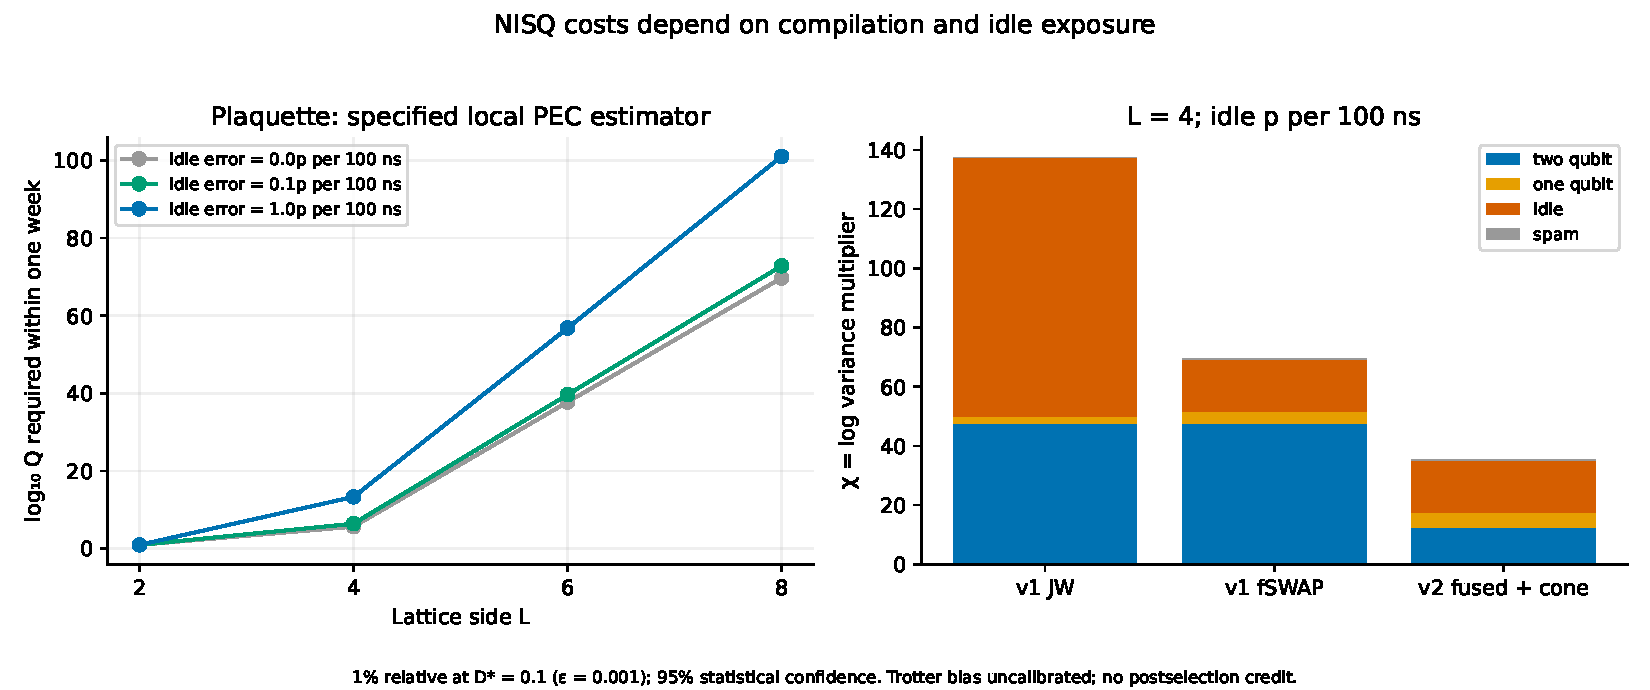
\includegraphics[width=\linewidth]{results/nisq_v2/nisq_resources.pdf}
\caption{Conditional PEC costs and their exposure decomposition. The precision
is $\eps=0.001$, with half allocated to statistical error. The idle sensitivities
keep the compiled circuit fixed. No postselection improvement is credited,
and the reserved Trotter error has not been verified.}
\end{figure}

\section{Postselection: exact acceptance, unresolved observable bias}
We first implement selection on the two spin parities
$P_\sigma=(-1)^{N_\sigma}$, not exact particle-number selection.
For the compiled circuits, each of the three characters
$P_\uparrow,P_\downarrow,P_\uparrow P_\downarrow$ remains a single Pauli under
backwards propagation through every primitive. This is checked explicitly;
the shortcut rejects a non-Clifford gate that would spread a character.

Each independent depolarizing location multiplies a character by $s_k$ if
its restriction to that location is nonidentity, and by one otherwise.
Preparation and readout flips contribute $1-2p$ on the relevant wires.
Let $\Lambda_\sigma$ be the product of these factors, normalized to the ideal
parity eigenvalue. The exact acceptance is then
\begin{equation}
 A=\frac14\left(1+\Lambda_\uparrow+\Lambda_\downarrow+
 \Lambda_{\uparrow\downarrow}\right).
\end{equation}
This derivation includes the primitive gate basis and the scheduled idle
intervals. It assumes neither that errors occur at Gaussian-block boundaries
nor that the noisy state is a classical occupation distribution.

At $L=4$, we obtain $A=0.2505$ for the refined plaquette circuit. The fully
randomized parity limit is $1/4$, so a nonvanishing acceptance says little by
itself about the retained state. If $P_0$ is the probability of no faults,
the only state-independent conditional bias guarantee we currently use is
\begin{equation}
 |D_{\mathrm{selected}}-D_{\mathrm{ideal}}|
 \leq 1-P_0/A.
\end{equation}
It follows by separating the accepted no-fault component from all accepted
faulty components, with $0\leq D\leq1$. At $L=4$ this bound is $0.9997$;
even at $L=2$ it is about $0.123$. These loose sufficient bounds do not
measure the actual bias, but they do not certify $\eps=0.001$.

Exact spin-resolved particle-number selection is stronger and remains to be
implemented for the noisy estimator. Its maximally mixed benchmark illustrates
the same distinction: for $N=L^2$ sites at half filling,
\begin{equation}
 A_{N_\uparrow=N_\downarrow=N/2}
 =\left[2^{-N}{N\choose N/2}\right]^2\sim\frac{2}{\pi N},
 \qquad D_{\mathrm{selected}}=\frac14.
\end{equation}
Polynomial acceptance alone therefore does not restore an arbitrary target
doublon expectation. We have not multiplied PEC overhead by $1/A$ and called
the result a corrected estimator: combining PEC with conditioning requires
its own numerator/denominator and bias analysis.

\begin{figure}[t]
\centering
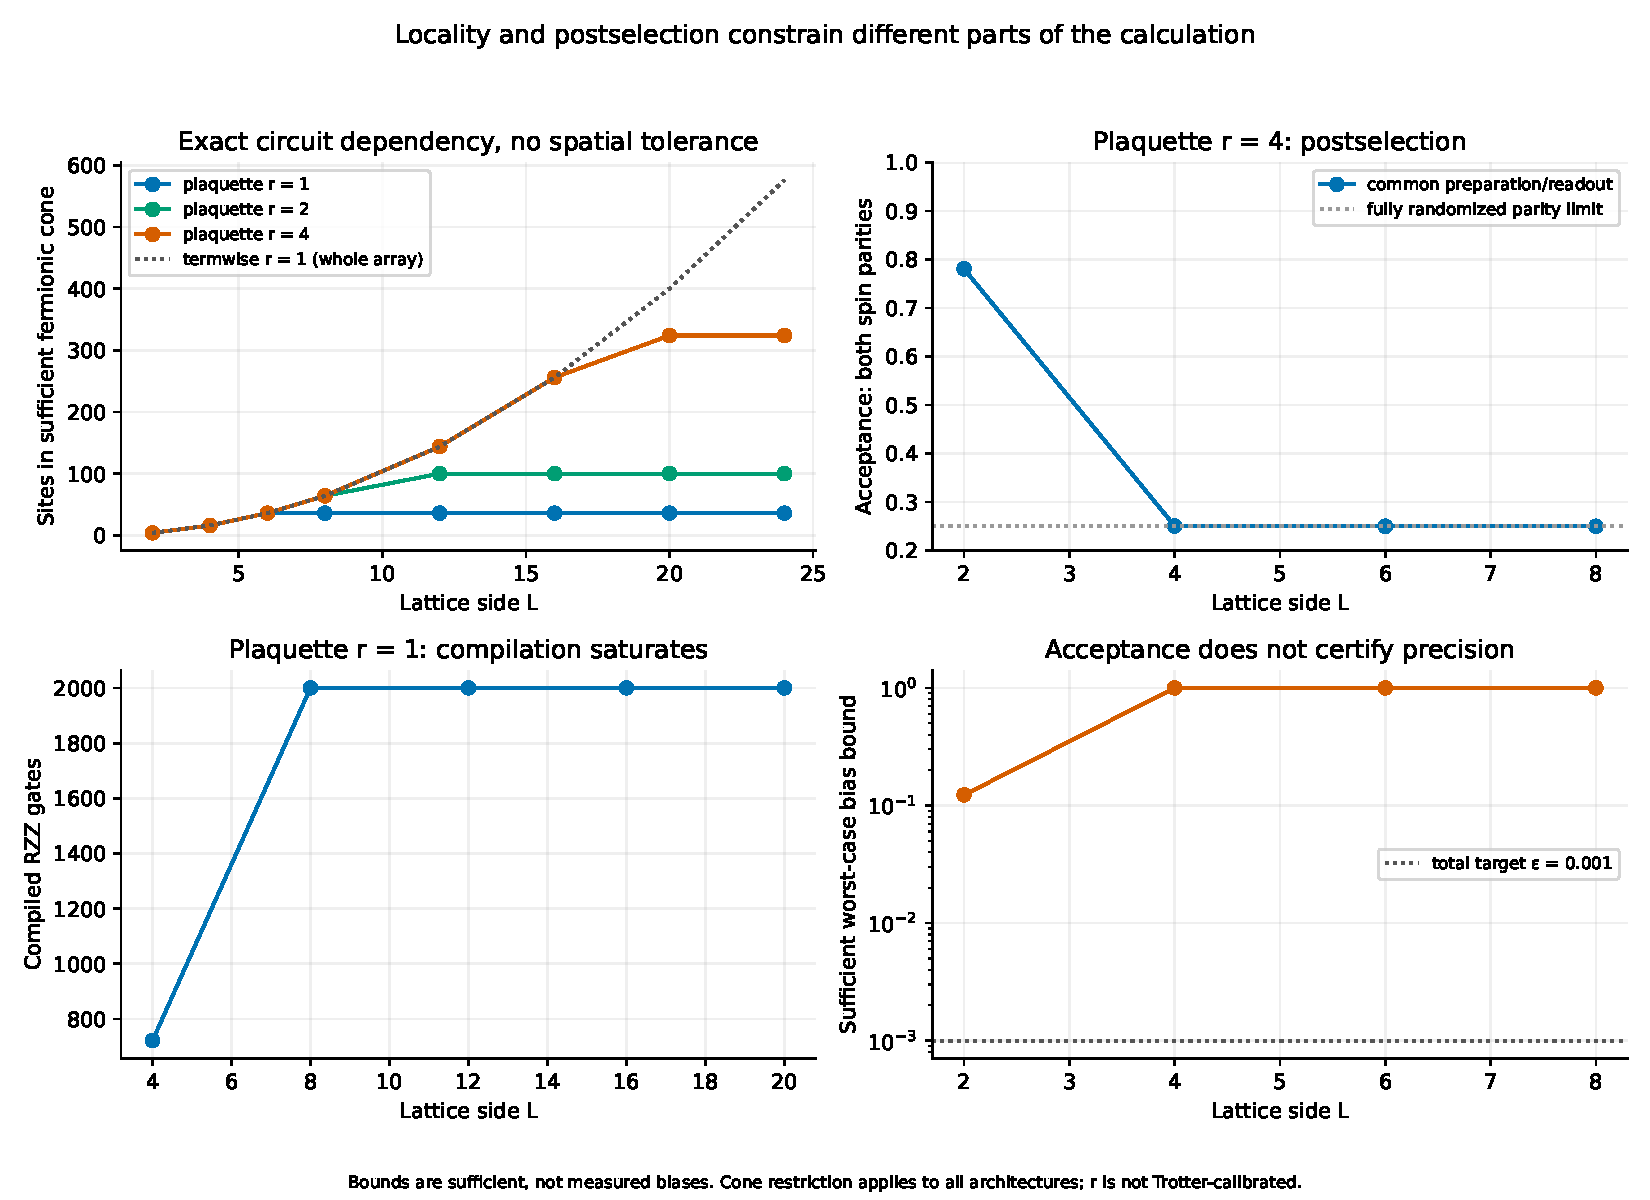
\includegraphics[width=\linewidth]{results/nisq_v2/locality_postselection.pdf}
\caption{Sufficient circuit cones, compiled cost saturation at fixed $r$, and
spin-parity postselection. The final panel is a worst-case bias upper bound,
not a measured bias or a lower bound. The strict termwise dependency cone
should not be confused with a finite-tolerance Hamiltonian light cone.}
\end{figure}

\section{Injected-state error changes the hybrid result}
The distillation input is an injected-state error $p_{\mathrm{in}}$, separate
from the physical circuit error $p$. For the retained leading-order serial
15-to-1 reference~\cite{litinski},
\begin{equation}
 p_1=35p_{\mathrm{in}}^3,\quad a_1=1-15p_{\mathrm{in}},\qquad
 p_2=35p_1^3,\quad a_2=1-15p_1.
\end{equation}
We keep the same 12-tile one-level and 37-tile serial two-level factory
references, replacing only the input error and corresponding acceptance.
The physical surface-code error law still uses $p=10^{-3}$.

Akahoshi et al. quote conventional injection coefficients $46/15$ and
$34/15$, and use $46p/15$ in their FT comparison~\cite{akahoshi}.
These coefficients depend on the injection circuit and its noise model;
we have not recalibrated them for our asymmetric $p_{1q}=p/10$ convention.
They define source-backed input-quality scenarios here.
Using $p_{\mathrm{in}}=46p/15$ gives $p_1\simeq1.009\times10^{-6}$,
about $28.8$ times the old $35p^3$. At $L=4$, $576$ fixed-angle states then
exceed the hybrid magic-error budget, even before its PEC amplification.
Two-level distillation is required in the current model.

\begin{center}
\begin{tabular}{lrr}
\toprule
$L=4$, $\eps=0.001$ & $p_{\mathrm{in}}=p$ & $p_{\mathrm{in}}=46p/15$\\
\midrule
All-angle STAR area & 166698 & 166698\\
Hybrid area & 66150 & 669714\\
Hybrid distillation levels & 1 & 2\\
FT area & 13791250 & 13791250\\
\bottomrule
\end{tabular}
\end{center}
Thus the earlier $2.52$-fold hybrid improvement reverses at this point under
conventional injection and the serial factory reference. The benefit survives
at $L=8$ at about $7.3$-fold. Replica rounding is not the whole explanation:
relaxing replica integrality for the selected configurations gives about
$1.30\times10^5$ qubits for all-angle STAR and $5.25\times10^5$ for the
corrected hybrid at $L=4$.

Precision and injection quality must be varied jointly. At $\eps=0.01$,
one-level FT passes with $p_{\mathrm{in}}=p$, but still fails with
$p_{\mathrm{in}}=46p/15$. The hybrid passes with one level at this looser
precision in both cases. This sensitivity holds the more accurate compiled
FT words fixed, so re-synthesis could further reduce the looser-precision cost.
The actual v1 fit was 70 T gates per dynamic rotation; counting the fixed
gates as well gives 72 per dynamic rotation. GridSynth gave 66 dynamic T gates.

There is a further architecture choice: Akahoshi's postselected prepared-state
error is $2p/15+O(p^2)$, while the $4p/15$ rotation error includes repeat-until-success
consumption~\cite{akahoshi}. Feeding the better prepared state into distillation
can change both FT and hybrid factory levels. We include $2p/15$ as a conditional
sensitivity, but have not charged a compiled implementation of its injection
acceptance and supply. A fair optimized comparison must allow FT to use improved
injection too; a single input-error coefficient is not an architecture law.

\begin{figure}[t]
\centering
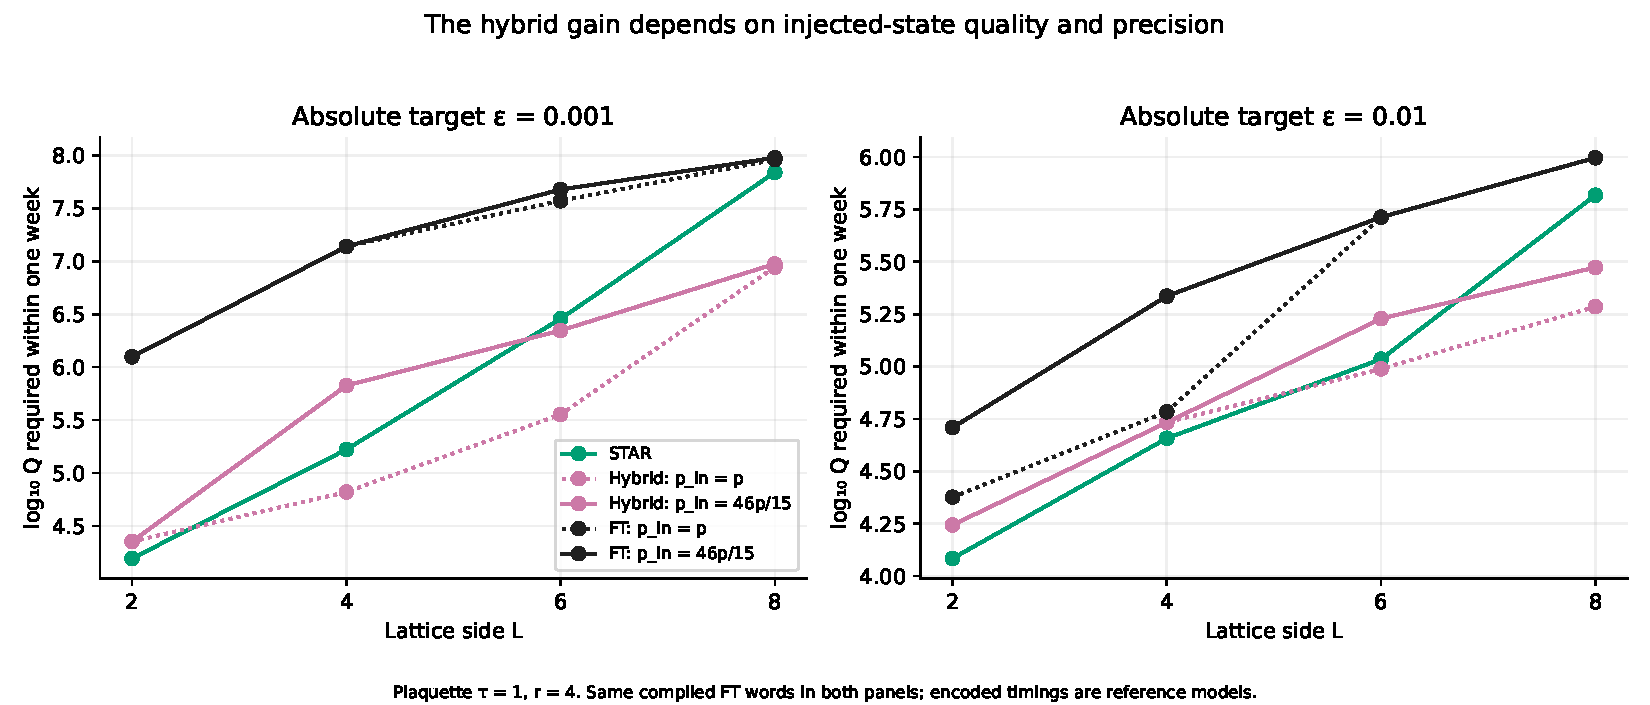
\includegraphics[width=\linewidth]{results/nisq_v2/factory_reassessment.pdf}
\caption{Factory switching changes the hybrid result. Both panels use the
compiled FT words for $\eps=0.001$; the right panel isolates looser error
allocation and sampling. Timing, tile counts, logical-error fits, and serial
factory supply remain the declared encoded reference models.}
\end{figure}

\section{Scope of the completed refinement}
The new native circuits compile in CUDA-Q Logical without using the rejected
encoded backend schedule. Local matrix identities verify Gaussian fusion,
fermionic permutations, parity trees, and cone compression. An independent
two-mode density-channel calculation checks parity acceptance with every native
fault location, including idle and boundary timing. These are local circuit
and channel checks, not a many-body dynamics calibration.

The remaining NISQ work is a better topology-aware ordering, exact
particle-number selection and its residual observable bias, and a calibrated
combined mitigation estimator. STAR injection/growth/retry schedules and the
encoded scheduling reproducer remain the next architecture tasks. The C9
commuting-Pauli sensitivity is retained; its use as a STAR default still
requires a residual-channel and branch-dependence argument for those gadgets.
Trotter calibration and qubitization retain their later position.

\bibliographystyle{unsrt}
\bibliography{references,refinement_references}
\end{document}
